\documentclass[aspectratio=169,12pt,t]{beamer}

% --- Theme: Metropolis (modern, clean) ---
\usetheme[progressbar=frametitle,numbering=fraction,block=fill]{metropolis}

% --- Fira Sans font (install texlive-fonts-extra if missing) ---
\IfFileExists{FiraSans.sty}{\usepackage[sfdefault]{FiraSans}}{}

% --- Light background with warm accent ---
\definecolor{mDarkTeal}{RGB}{35,55,59}
\definecolor{mLightBrown}{RGB}{235,228,216}
\definecolor{mAccent}{RGB}{140,70,20}

\setbeamercolor{normal text}{fg=mDarkTeal,bg=white}
\setbeamercolor{alerted text}{fg=mAccent}
\setbeamercolor{frametitle}{bg=mDarkTeal,fg=white}
\setbeamercolor{progress bar}{fg=mAccent,bg=mLightBrown}
\setbeamercolor{title separator}{fg=mAccent}
\setbeamercolor{progress bar in head/foot}{fg=mAccent,bg=mLightBrown}
\setbeamercolor{progress bar in section page}{fg=mAccent,bg=mLightBrown}

% --- Packages ---
\usepackage[utf8]{inputenc}
\usepackage{amsmath,amssymb,amsthm}
\usepackage{mathrsfs}
\usepackage{tikz}
\usetikzlibrary{arrows.meta,positioning,calc,decorations.pathreplacing,shapes,patterns}
\usepackage{pgfplots}
\pgfplotsset{compat=1.18}

% --- Semi-transparent white highlight for text on top of background images ---
\usepackage[most]{tcolorbox}

% Inline highlight: \hl{short text}
\newtcbox{\hl}{%
  nobeforeafter, tcbox raise base,
  colback=white, opacityback=0.6,
  colframe=white, opacityframe=0,
  sharp corners, boxsep=2pt, left=3pt, right=3pt, top=2pt, bottom=2pt%
}

% Block highlight: \begin{hlbox} ... \end{hlbox}  (multi-line, paragraphs, itemize)
\newtcolorbox{hlbox}[1][]{%
  enhanced, breakable,
  colback=white, opacityback=0.6,
  colframe=white, opacityframe=0,
  boxsep=3pt, left=6pt, right=6pt, top=4pt, bottom=4pt,
  sharp corners,
  {#1}%
}

% --- Custom colors for content types ---
\definecolor{defcolor}{RGB}{25,85,120}
\definecolor{thmcolor}{RGB}{140,35,35}
\definecolor{proofcolor}{RGB}{35,100,50}
\definecolor{excolor}{RGB}{140,75,10}
\definecolor{remcolor}{RGB}{90,90,90}

% --- Beamer blocks for mathematical content types (semi-transparent) ---
\tcbset{hlblockbase/.style={
  enhanced, breakable,
  coltitle=white, fonttitle=\bfseries,
  opacitybacktitle=0.8, opacityback=0.6,
  opacityframe=0,
  sharp corners,
  boxsep=1pt, left=5pt, right=5pt, top=2pt, bottom=2pt,
  toptitle=1pt, bottomtitle=1pt
}}

\newtcolorbox{defblock}[1]{hlblockbase, title={#1},
  colbacktitle=defcolor, colback=defcolor!15, colframe=defcolor}
\newtcolorbox{thmblock}[1]{hlblockbase, title={#1},
  colbacktitle=thmcolor, colback=thmcolor!15, colframe=thmcolor}
\newtcolorbox{proofblock}[1]{hlblockbase, title={#1},
  colbacktitle=proofcolor, colback=proofcolor!15, colframe=proofcolor}
\newtcolorbox{exblock}[1]{hlblockbase, title={#1},
  colbacktitle=excolor, colback=excolor!15, colframe=excolor}
\newtcolorbox{remblock}[1]{hlblockbase, title={#1},
  colbacktitle=remcolor, colback=remcolor!15, colframe=remcolor}

% --- Metadata ---
\title{Chapter 3: Numerical Sequences and Series}
\subtitle{Section: Series of Nonnegative Terms}
\author{Based on Walter Rudin's \emph{Principles of Mathematical Analysis}}
\date{}

\begin{document}

% =============================================================================
% TITLE AND OUTLINE
% =============================================================================
{
\usebackgroundtemplate{%
  
\includegraphics[width=\paperwidth,height=\paperheight,keepaspectratio=false]{chapter_03_bg_00.png}%
}
\begin{frame}[plain]
  \titlepage
  \note{
    Welcome back to Chapter 3 of Principles of Mathematical Analysis.
    In the previous section we set up the general theory of infinite
    series: partial sums, the Cauchy criterion, the divergence test,
    and the comparison test. The comparison test told us that to
    decide whether a series converges, it helps to compare it to a
    series whose behaviour we already understand. In this section we
    stock our toolbox with the most important reference series for
    nonnegative-term comparisons. We will prove four results: the
    geometric series, the Cauchy condensation test, the "p"-series
    test, and a refinement involving logarithms. Together these
    cover almost every nonnegative-term series you will meet in
    practice.
  }
\end{frame}
}

{
\usebackgroundtemplate{%
  
\includegraphics[width=\paperwidth,height=\paperheight,keepaspectratio=false]{chapter_03_bg_01.png}%
}
\begin{frame}[c]{Outline}
  \begin{center}
    \tableofcontents
  \end{center}
  \note{
    Here is the plan. We open with motivation: why nonnegative-term
    series are special and what we hope to gain from the section.
    The first stop is the geometric series, Theorem 3.26, our most
    basic reference series. We then turn to Theorem 3.27, the Cauchy
    condensation test, which lets us decide convergence by looking
    at a thin subsequence of the original series. We apply the
    condensation test twice: first to get Theorem 3.28, the
    "p"-series test, and then to get Theorem 3.29, the logarithmic
    series test. We close with a brief discussion of the so-called
    boundary between convergent and divergent series, and a summary
    of what we have built.
  }
\end{frame}

% =============================================================================
% MOTIVATION
% =============================================================================
\section{Motivation}

% --- Build 1/4 ---
\begin{frame}{Why Nonnegative Terms?}
  \begin{hlbox}
  \begin{itemize}
    \item Comparison test (Theorem 3.25) needs \alert{reference series} we trust
  \end{itemize}
  \end{hlbox}

  \note{
    Recall the comparison test from the previous section. To prove
    that a series converges or diverges, we compare it term-by-term
    to a series whose behaviour is already known. The whole strategy
    is only useful if we have a stockpile of reference series whose
    behaviour we have nailed down. Building that stockpile is what
    this section is about.
  }
\end{frame}

% --- Build 2/4 ---
\begin{frame}{Why Nonnegative Terms?}
  \begin{hlbox}
  \begin{itemize}
    \item Comparison test (Theorem 3.25) needs \alert{reference series} we trust
    \item For $a_n \geq 0$, partial sums $\{s_n\}$ are \emph{monotonically increasing}
  \end{itemize}
  \end{hlbox}

  \note{
    Nonnegative terms have one big technical advantage. If every
    term is at least zero, then each new partial sum is at least as
    large as the previous one, so the sequence of partial sums is
    monotonically increasing. Monotone sequences are much easier to
    handle than general sequences: they converge if and only if they
    are bounded above.
  }
\end{frame}

% --- Build 3/4 ---
\begin{frame}{Why Nonnegative Terms?}
  \begin{hlbox}
  \begin{itemize}
    \item Comparison test (Theorem 3.25) needs \alert{reference series} we trust
    \item For $a_n \geq 0$, partial sums $\{s_n\}$ are \emph{monotonically increasing}
    \item By Theorem 3.24: convergence $\;\Longleftrightarrow\;$ partial sums \alert{bounded}
  \end{itemize}
  \end{hlbox}

  \note{
    This is exactly Theorem 3.24 from the previous section: a series
    of nonnegative terms converges if and only if its partial sums
    form a bounded sequence. This single fact removes all the
    epsilon-machinery and turns convergence questions into bounded
    questions. It is the workhorse behind every proof in this
    section.
  }
\end{frame}

% --- Build 4/4 ---
\begin{frame}{Why Nonnegative Terms?}
  \begin{hlbox}
  \begin{itemize}
    \item Comparison test (Theorem 3.25) needs \alert{reference series} we trust
    \item For $a_n \geq 0$, partial sums $\{s_n\}$ are \emph{monotonically increasing}
    \item By Theorem 3.24: convergence $\;\Longleftrightarrow\;$ partial sums \alert{bounded}
    \item Goal: nail down \alert{four reference series} as benchmarks
  \end{itemize}
  \end{hlbox}

  \note{
    Our goal in this section is to nail down four families of
    reference series. The geometric series, the condensation
    principle, the "p"-series, and the logarithmic series. The first
    is concrete and classical; the second is a powerful general
    tool; the third and fourth are applications of the second. With
    these in hand, almost any nonnegative-term series you meet in
    practice can be decided by comparison. Let us begin with the
    simplest example.
  }
\end{frame}
}

{
\usebackgroundtemplate{%
  
\includegraphics[width=\paperwidth,height=\paperheight,keepaspectratio=false]{chapter_03_bg_02.png}%
}
% =============================================================================
% THE GEOMETRIC SERIES
% =============================================================================
\section{The Geometric Series}

% --- Hook ---
\begin{frame}{The Simplest Series of All}
  \begin{center}
    \hl{$1 + x + x^2 + x^3 + x^4 + \cdots$}
  \end{center}

  \vspace{0.6em}
  \begin{hlbox}
    \textbf{Question:} When does this infinite sum make sense, and what is its value?
    \vspace{0.6em}

    \textbf{Idea:} the partial sum $1 + x + \cdots + x^n$ has a closed form.
  \end{hlbox}

  \note{
    The geometric series is the most basic infinite series in all
    of analysis. The terms are powers of a fixed number "x". We
    want to know two things: for which values of "x" does the
    series converge, and when it does, what is the sum? The reason
    the geometric series is tractable is that its partial sums have
    a clean closed form: 1 plus "x" plus "x" squared all the way to
    "x" to the "n" can be written as a single fraction, with no
    summation symbol. From there the limit is straightforward.
  }
\end{frame}

% --- Theorem 3.26 statement ---
\begin{frame}{Theorem 3.26: The Geometric Series}
  \begin{thmblock}{Theorem 3.26}
    If $0 \leq x < 1$, then
    \[
      \sum_{n=0}^{\infty} x^n \;=\; \frac{1}{1 - x} .
    \]
    If $x \geq 1$, the series diverges.
  \end{thmblock}

  \vspace{0.6em}
  \begin{hlbox}
  \begin{itemize}
    \item Convergent for $0 \leq x < 1$, with explicit sum
    \item Divergent for $x \geq 1$
  \end{itemize}
  \end{hlbox}

  \note{
    Here is the statement. For "x" between 0 and 1, not including
    1, the geometric series converges and its sum is one over one
    minus "x". For "x" greater than or equal to 1, the series
    diverges. Notice the asymmetry of the conclusion: when it
    converges, we do not just know it converges, we have an exact
    formula for the limit. That makes the geometric series an
    especially useful reference for comparison arguments.
  }
\end{frame}

% --- Proof strategy ---
\begin{frame}{Proof Strategy}
  \hl{\textbf{Goal:} understand $\displaystyle s_n = \sum_{k=0}^{n} x^k = 1 + x + x^2 + \cdots + x^n$.}

  \vspace{0.8em}
  \begin{hlbox}
  \textbf{Plan:}
  \begin{enumerate}
    \item Find a \alert{closed form} for $s_n$ when $x \neq 1$.
    \item Take $n \to \infty$ to read off the sum.
    \item Treat $x = 1$ separately by inspection.
  \end{enumerate}
  \end{hlbox}

  \note{
    The plan is short and concrete. First, we compute a closed
    form for the partial sum "s" sub "n" when "x" is not equal to
    1, using a standard algebraic trick. Second, we let "n" go to
    infinity in that closed form, which immediately tells us
    whether and to what the series converges. Third, the case "x"
    equals 1 has to be handled separately because the closed-form
    fraction has a zero in the denominator there; but in that case
    the series is just 1 plus 1 plus 1 forever, which obviously
    diverges.
  }
\end{frame}

% --- Proof Step 1: closed form ---
\begin{frame}{Proof --- Step 1: A Closed Form}
  \begin{proofblock}{Closed form for the partial sum}
    For $x \neq 1$,
    \[
      s_n \;=\; \sum_{k=0}^{n} x^k \;=\; \frac{1 - x^{n+1}}{1 - x} .
    \]
  \end{proofblock}

  \vspace{0.5em}
  \hl{\textbf{Check:} $(1 - x)\,(1 + x + x^2 + \cdots + x^n) = 1 - x^{n+1}$ (telescoping).}

  \note{
    Step 1 gives us a closed form for the partial sum. The trick is
    the telescoping identity highlighted on the slide. Multiply the
    partial sum by 1 minus "x" and distribute: you get the sum 1
    plus "x" plus "x" squared up to "x" to the "n", minus the same
    sum shifted up by one power. Every middle power of "x" appears
    once with a plus sign and once with a minus sign, so it
    cancels. What survives is just the 1 from the bottom of the
    first sum and the minus "x" to the "n" plus 1 from the top of
    the second. Dividing by 1 minus "x", which is nonzero since we
    assumed "x" is not 1, gives the formula on the slide. The
    entire partial sum is now captured by a single fraction, and
    that is the only real computation in the whole proof.
  }
\end{frame}

% --- Proof Step 2: take the limit ---
\begin{frame}{Proof --- Step 2: Let $n \to \infty$}
  \begin{proofblock}{Case $0 \leq x < 1$}
    Then $x^{n+1} \to 0$ as $n \to \infty$, so
    \[
      s_n \;=\; \frac{1 - x^{n+1}}{1 - x} \;\longrightarrow\; \frac{1}{1 - x} .
    \]
  \end{proofblock}

  \vspace{0.6em}
  \begin{proofblock}{Case $x > 1$}
    Then $x^{n+1} \to \infty$, so $s_n \to \infty$ and the series diverges.
  \end{proofblock}

  \note{
    Step 2 is where the limit actually happens. We let "n" grow
    without bound in the closed form from Step 1, and notice that
    the whole expression is controlled by a single moving part:
    the power "x" to the "n" plus 1 sitting in the numerator. When
    "x" lies between 0 and 1, repeatedly multiplying by a number
    smaller than 1 drives that power to zero. This is one of the
    special limits we established earlier in the chapter. So the
    numerator settles down to 1 and the fraction approaches 1 over
    1 minus "x", which is exactly the sum claimed in the theorem.
    When "x" is greater than 1, the same power instead grows
    without bound, so the partial sums run off to infinity and the
    series diverges. The only value still untreated is the
    boundary case "x" equals 1, and we turn to it next.
  }
\end{frame}

% --- Proof Step 3: x = 1 case ---
\begin{frame}{Proof --- Step 3: The Case $x = 1$}
  \begin{proofblock}{Case $x = 1$}
    The series becomes
    \[
      1 + 1 + 1 + 1 + \cdots ,
    \]
    so $s_n = n + 1 \to \infty$.
    \alert{Divergent.} \hfill $\square$
  \end{proofblock}

  \vspace{0.6em}
  \hl{Every case covered: convergent for $0 \leq x < 1$, divergent for $x \geq 1$.}

  \note{
    Step 3 is the boundary case "x" equals 1, which the closed-form
    formula does not handle because the denominator vanishes there.
    But we do not need any machinery: each term is just 1, the
    partial sums are 1, 2, 3, 4, and so on, and they go to
    infinity. The series obviously diverges. Combining the three
    cases, we have proved the theorem: the geometric series
    converges precisely when "x" is strictly less than 1, with sum
    1 over 1 minus "x".
  }
\end{frame}

% --- Visualization ---
\begin{frame}{Geometric Series: $x = \tfrac{1}{2}$}
  \begin{center}
  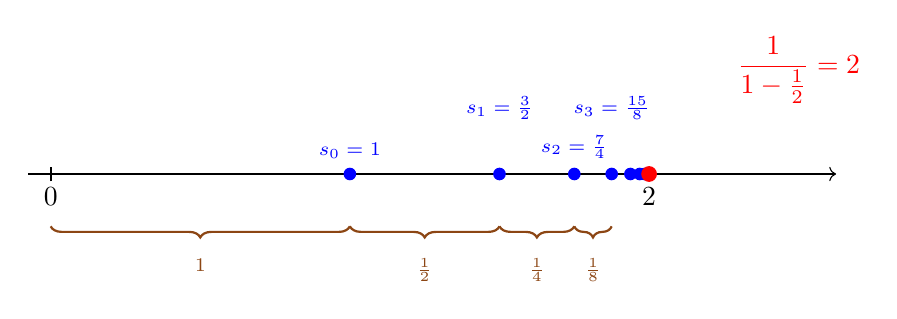
\begin{tikzpicture}[scale=0.95]
    % Axes
    \draw[->] (-0.3,0) -- (10.5,0) node[right]{};
    \node[below] at (0,-0.05) {$0$};
    \node[below] at (8,-0.05) {$2$};
    \draw[thick] (8,-0.1) -- (8,0.1);
    \draw[thick] (0,-0.1) -- (0,0.1);

    % Mark partial sums s_n on the axis
    \def\xhalf{0.5}
    % s_0 = 1
    \fill[blue] (4,0) circle (2.4pt) node[above=2pt]{\scriptsize $s_0=1$};
    % s_1 = 1.5
    \fill[blue] (6,0) circle (2.4pt) node[above=16pt]{\scriptsize $s_1=\tfrac{3}{2}$};
    % s_2 = 1.75
    \fill[blue] (7,0) circle (2.4pt) node[above=2pt]{\scriptsize $s_2=\tfrac{7}{4}$};
    % s_3 = 1.875
    \fill[blue] (7.5,0) circle (2.4pt) node[above=16pt]{\scriptsize $s_3=\tfrac{15}{8}$};
    % s_4 = 1.9375
    \fill[blue] (7.75,0) circle (2.4pt);
    \fill[blue] (7.875,0) circle (2.4pt);
    \fill[blue] (7.9375,0) circle (2.4pt);

    % Limit point
    \fill[red] (8,0) circle (3pt);
    \node[red, above=22pt] at (10,0) {$\dfrac{1}{1-\tfrac{1}{2}} = 2$};

    % Brackets showing successive halves
    \draw[thick, mAccent, decorate, decoration={brace, amplitude=4pt, mirror}] (0,-0.7) -- (4,-0.7) node[midway, below=8pt]{\scriptsize $1$};
    \draw[thick, mAccent, decorate, decoration={brace, amplitude=4pt, mirror}] (4,-0.7) -- (6,-0.7) node[midway, below=8pt]{\scriptsize $\tfrac{1}{2}$};
    \draw[thick, mAccent, decorate, decoration={brace, amplitude=4pt, mirror}] (6,-0.7) -- (7,-0.7) node[midway, below=8pt]{\scriptsize $\tfrac{1}{4}$};
    \draw[thick, mAccent, decorate, decoration={brace, amplitude=4pt, mirror}] (7,-0.7) -- (7.5,-0.7) node[midway, below=8pt]{\scriptsize $\tfrac{1}{8}$};
  \end{tikzpicture}
  \end{center}

  \vspace{0.4em}
  \begin{center}
    \hl{Each term covers \emph{half} of the remaining gap to $2$.}
  \end{center}

  \note{
    Here is the geometric series with "x" equal to one half pictured
    on the number line. The blue dots are successive partial sums:
    the first is 1, then 1 and a half, then 1 and three quarters,
    then 1 and seven eighths, and so on. The red dot at 2 is the
    limit, since 1 over 1 minus one half equals 2. The orange
    brackets below the axis show how each new term covers exactly
    half of the remaining gap to 2. This picture makes Zeno's
    paradox feel almost obvious in hindsight: you never finish the
    walk in any finite step, but you do approach the destination as
    a limit.
  }
\end{frame}

% --- Examples ---
\begin{frame}{Two Quick Applications}
  \begin{exblock}{Geometric series in action}
    \begin{itemize}
      \item $\displaystyle 1 + \tfrac{1}{2} + \tfrac{1}{4} + \tfrac{1}{8} + \cdots
        = \frac{1}{1 - 1/2} = 2$
      \item $\displaystyle \sum_{n=0}^{\infty} \frac{1}{3^n}
        = \frac{1}{1 - 1/3} = \frac{3}{2}$
    \end{itemize}
  \end{exblock}

  \vspace{0.6em}
  \begin{hlbox}
    \textbf{Why we care:} the geometric series is the universal yardstick for the comparison and root/ratio tests to come.
  \end{hlbox}

  \note{
    Two quick numerical examples. With "x" equal to one half, the
    sum is 1 over 1 minus one half, which is 2. With "x" equal to
    one third, the sum is 1 over 1 minus one third, which is three
    halves. Both fall out of the formula instantly. The geometric
    series will appear constantly throughout the rest of the
    chapter, especially when we prove the root test and the ratio
    test. Whenever we want to show a series converges fast, the
    standard move is to compare it term-by-term to a geometric
    series with ratio strictly less than 1.
  }
\end{frame}
}

{
\usebackgroundtemplate{%
  
\includegraphics[width=\paperwidth,height=\paperheight,keepaspectratio=false]{chapter_03_bg_03.png}%
}
% =============================================================================
% CAUCHY CONDENSATION TEST
% =============================================================================
\section{Cauchy Condensation Test}

% --- Hook 1 ---
\begin{frame}{A Stronger Tool for Monotone Series}
  \begin{hlbox}
  \begin{itemize}
    \item Suppose the terms \alert{decrease monotonically}:
      $a_1 \geq a_2 \geq a_3 \geq \cdots \geq 0$.
    \item In applications, this is the \emph{typical} situation.
  \end{itemize}
  \end{hlbox}

  \vspace{0.6em}
  \hl{\textbf{Question:} can we test convergence using only a few sample terms?}

  \note{
    Most nonnegative-term series you meet in practice have the
    extra property that the terms are decreasing: the second term
    is no bigger than the first, the third is no bigger than the
    second, and so on, all the way down to zero. In that monotone
    setting we can do something surprising. We can decide
    convergence by looking only at a thin subsequence of the
    original terms, sampled at powers of 2. That is the content of
    Cauchy's condensation test, which we state next.
  }
\end{frame}

% --- Theorem 3.27 ---
\begin{frame}{Theorem 3.27: Cauchy Condensation Test}
  \begin{thmblock}{Theorem 3.27}
    Suppose $a_1 \geq a_2 \geq a_3 \geq \cdots \geq 0$. Then the series
    $\displaystyle \sum_{n=1}^{\infty} a_n$ converges if and only if
    \[
      \sum_{k=0}^{\infty} 2^k a_{2^k}
      \;=\; a_1 + 2 a_2 + 4 a_4 + 8 a_8 + 16 a_{16} + \cdots \tag{7}
    \]
    converges.
  \end{thmblock}

  \vspace{0.5em}
  \hl{Striking feature: a \alert{very thin} subsequence determines convergence.}

  \note{
    Here is the theorem. We assume the terms "a" sub "n" are
    nonnegative and weakly decreasing. The claim is that the
    original series and the condensed series, which uses only the
    first, second, fourth, eighth, sixteenth, and so on terms, each
    multiplied by the matching power of 2, both converge or both
    diverge. The striking feature is just how thin the condensed
    sample is. Even though the condensed series only inspects
    terms at the powers of 2, it captures the full convergence
    behaviour of the original series. The proof is short and uses
    nothing more than careful grouping.
  }
\end{frame}

% --- Intuition diagram ---
\begin{frame}{Intuition: Grouping by Powers of $2$}
  \begin{hlbox}
  \textbf{Upper bound} --- blocks \emph{starting} at $2^k$, each term $\leq$ first term:
  \[
    a_1 + \underbrace{(a_2 + a_3)}_{\leq\, 2 a_2}
        + \underbrace{(a_4 + \cdots + a_7)}_{\leq\, 4 a_4}
        + \underbrace{(a_8 + \cdots + a_{15})}_{\leq\, 8 a_8} + \cdots
  \]

  \vspace{0.4em}
  \textbf{Lower bound} --- blocks \emph{ending} at $2^k$, each term $\geq$ last term:
  \[
    a_1 + a_2 + \underbrace{(a_3 + a_4)}_{\geq\, 2 a_4}
              + \underbrace{(a_5 + \cdots + a_8)}_{\geq\, 4 a_8}
              + \underbrace{(a_9 + \cdots + a_{16})}_{\geq\, 8 a_{16}} + \cdots
  \]

  \vspace{0.3em}
  Both groupings reproduce $a_1 + 2 a_2 + 4 a_4 + 8 a_8 + \cdots$ up to a factor of $2$.
  \end{hlbox}

  \note{
    Here is the picture behind the proof. Two slightly different
    groupings do all the work. For the upper bound, shown on the
    top line, we group the terms into blocks that start at a power
    of 2: a single term "a" sub 1, then the block of length 2
    starting at "a" sub 2, then the block of length 4 starting at
    "a" sub 4, and so on. Because the sequence is decreasing, every
    term in such a block is at most its first term, so each block
    of length 2 to the "k" is bounded above by 2 to the "k" copies
    of "a" sub 2 to the "k". Reading off the bounds gives the
    condensed series exactly.

    For the lower bound on the second line, we shift the grouping
    by one step so each block ends at a power of 2 instead of
    starting at one. Now every term is at least the last term, and
    the block sums are bounded below by 2 times "a" sub 4, then 4
    times "a" sub 8, then 8 times "a" sub 16, and so on. Reading
    off these bounds gives the same condensed series, now shifted
    by one place. Both groupings, upper and lower, reproduce the
    condensed series up to a factor of 2. That two-sided sandwich
    is the whole proof.
  }
\end{frame}

% --- Proof setup ---
\begin{frame}{Proof --- Setup}
  \begin{proofblock}{Two partial sums}
    \begin{align*}
      s_n &= a_1 + a_2 + \cdots + a_n , \\
      t_k &= a_1 + 2 a_2 + 4 a_4 + \cdots + 2^k a_{2^k} .
    \end{align*}
  \end{proofblock}

  \vspace{0.6em}
  \begin{hlbox}
    By Theorem 3.24, both series converge iff their partial sums are bounded.
  \end{hlbox}

  \vspace{0.4em}
  \hl{\textbf{Strategy:} show $\{s_n\}$ bounded $\;\Longleftrightarrow\;$ $\{t_k\}$ bounded.}

  \note{
    To prove the theorem we use Theorem 3.24, which says a
    nonnegative-term series converges if and only if its partial
    sums are bounded. So we just need to show that the partial sums
    of the original series are bounded if and only if the partial
    sums of the condensed series are bounded. Let "s" sub "n"
    denote the "n" th partial sum of the original series and "t"
    sub "k" denote the "k" th partial sum of the condensed series.
    The whole game is to bound "s" sub "n" by "t" sub "k" and vice
    versa.
  }
\end{frame}

% --- Proof Step 1 ---
\begin{frame}{Proof --- Step 1: $s_n \leq t_k$}
  \begin{proofblock}{Upper bound: $n < 2^{k+1}$}
    Grouping the first $n$ terms into blocks of length $1, 2, 4, \ldots, 2^k$:
    \begin{align*}
      s_n &\leq a_1 + (a_2 + a_3) + \cdots + (a_{2^k} + \cdots + a_{2^{k+1}-1}) \\
      &\leq a_1 + 2 a_2 + 4 a_4 + \cdots + 2^k a_{2^k} \;=\; t_k .
    \end{align*}
    Hence
    \[
      s_n \leq t_k . \tag{8}
    \]
  \end{proofblock}

  \note{
    Step 1. Pick any "n" and choose "k" large enough that 2 raised
    to the "k" plus 1 power exceeds "n". Group the first "n" terms
    into blocks of lengths 1, 2, 4, up to 2 to the "k". Inside each
    block of length 2 to the "j", every term is at most "a" sub 2
    to the "j", since the sequence is decreasing. So the block sum
    is at most 2 to the "j" times "a" sub 2 to the "j". Adding up
    all the block bounds gives exactly "t" sub "k". This is the
    first half of the sandwich: "s" sub "n" is at most "t" sub
    "k".
  }
\end{frame}

% --- Proof Step 2 ---
\begin{frame}{Proof --- Step 2: $2 s_n \geq t_k$}
  \begin{proofblock}{Lower bound: $n > 2^k$}
    Grouping again, but starting one step later:
    \begin{align*}
      s_n &\geq a_1 + a_2 + (a_3 + a_4) + \cdots + (a_{2^{k-1}+1} + \cdots + a_{2^k}) \\
      &\geq \tfrac{1}{2}\, a_1 + a_2 + 2 a_4 + \cdots + 2^{k-1} a_{2^k}
      \;=\; \tfrac{1}{2}\, t_k .
    \end{align*}
    Hence
    \[
      2 s_n \geq t_k . \tag{9}
    \]
  \end{proofblock}

  \note{
    Step 2 is the matching lower bound. Now choose "n" larger than
    2 to the "k". Group the first "n" terms into blocks of lengths
    1, 1, 2, 4, all the way up to 2 to the "k" minus 1. This time
    the smallest term in each block is its last term, so the block
    sum is at least its length times that last term. After this
    step we have a raw lower bound of "a" sub 1, plus "a" sub 2,
    plus 2 times "a" sub 4, plus 4 times "a" sub 8, and so on. To
    match the form of "t" sub "k", we deliberately weaken "a" sub
    1 down to half of itself; that costs nothing since "a" sub 1
    is nonnegative, and the surviving combination is precisely
    one half of "t" sub "k". Rearranging, twice the "n" th partial
    sum of the original series is at least "t" sub "k". That is
    the other half of the sandwich.
  }
\end{frame}

% --- Proof conclusion ---
\begin{frame}{Proof --- Conclusion}
  \begin{proofblock}{Combining (8) and (9)}
    From inequalities (8) and (9):
    \[
      s_n \leq t_k \quad\text{and}\quad t_k \leq 2 s_n .
    \]
    Therefore $\{s_n\}$ is bounded $\;\Longleftrightarrow\;$ $\{t_k\}$ is bounded.
  \end{proofblock}

  \vspace{0.5em}
  \hl{By Theorem 3.24, the two series converge or diverge \alert{together}.} \hfill $\square$

  \note{
    Combine the two inequalities. Either both sequences "s" sub "n"
    and "t" sub "k" are bounded, or both are unbounded; there is no
    third option, because each one bounds the other within a fixed
    multiplicative constant. By Theorem 3.24, boundedness is the
    same as convergence for these monotone partial sums. So the
    original series and the condensed series converge or diverge
    together. That completes the proof.
  }
\end{frame}
}

{
\usebackgroundtemplate{%
  
\includegraphics[width=\paperwidth,height=\paperheight,keepaspectratio=false]{chapter_03_bg_04.png}%
}
% =============================================================================
% THE P-SERIES
% =============================================================================
\section{The $p$-Series}

% --- Hook + Theorem ---
\begin{frame}{Theorem 3.28: The $p$-Series Test}
  \begin{thmblock}{Theorem 3.28}
    The series
    \[
      \sum_{n=1}^{\infty} \frac{1}{n^p}
    \]
    converges if $p > 1$ and diverges if $p \leq 1$.
  \end{thmblock}

  \vspace{0.6em}
  \begin{hlbox}
  \textbf{Two famous corner cases:}
  \begin{itemize}
    \item $p = 1$: the \alert{harmonic series} $\sum 1/n$ \alert{diverges}.
    \item $p = 2$: $\sum 1/n^2$ converges (the Basel problem: sum is $\pi^2/6$).
  \end{itemize}
  \end{hlbox}

  \note{
    The "p"-series test pins down exactly when the prototype series
    1 over "n" to the "p" converges. The answer is: it converges
    if "p" is strictly bigger than 1 and diverges if "p" is at
    most 1. Two cases are especially memorable. When "p" equals 1
    we get the harmonic series, 1 plus one half plus one third and
    so on, and the theorem says it diverges, even though the terms
    go to zero. When "p" equals 2 we get the Basel series, which
    Euler famously summed to pi squared over 6, though we will
    not need the exact value here.
  }
\end{frame}

% --- Proof Step 1 ---
\begin{frame}{Proof --- Step 1: The Easy Cases $p \leq 0$}
  \begin{proofblock}{Easy case: $p \leq 0$}
    If $p \leq 0$, then $n^{-p} \geq 1$ for all $n$, so $1/n^p \not\to 0$.

    \vspace{0.4em}
    By Theorem 3.23, the series \alert{diverges}.
  \end{proofblock}

  \vspace{0.6em}
  \hl{So from now on, assume $p > 0$.}

  \note{
    Step 1 disposes of the trivial range "p" less than or equal to
    0. In that case the exponent is at most zero, so 1 over "n" to
    the "p" is at least 1 for every "n". The terms do not even go
    to zero, so by Theorem 3.23, the divergence test, the series
    diverges. From here on, the interesting question is what
    happens for "p" positive.
  }
\end{frame}

% --- Proof Step 2 ---
\begin{frame}{Proof --- Step 2: Apply Cauchy Condensation}
  \begin{proofblock}{Condensation gives a geometric series}
    For $p > 0$, the sequence $\{1/n^p\}$ is positive and decreasing.
    Theorem 3.27 applies. The condensed series is
    \[
      \sum_{k=0}^{\infty} 2^k \cdot \frac{1}{2^{kp}}
      \;=\; \sum_{k=0}^{\infty} 2^{(1-p)k} .
    \]
  \end{proofblock}

  \vspace{0.4em}
  \hl{This is a \alert{geometric series} with ratio $x = 2^{1-p}$.}

  \note{
    Step 2. For "p" positive, the terms 1 over "n" to the "p" are
    positive and decreasing, so Cauchy's condensation test applies.
    Plug "a" sub 2 to the "k" equals 1 over 2 to the "k" "p" into
    the condensed sum on the slide. The factor of 2 to the "k"
    out front combines with the 1 over 2 to the "k" "p" inside to
    give 2 to the power 1 minus "p", times "k". So the condensed
    series is just a geometric series with ratio "x" equal to 2 to
    the power 1 minus "p".
  }
\end{frame}

% --- Proof Step 3 ---
\begin{frame}{Proof --- Step 3: Compare with the Geometric Series}
  \begin{proofblock}{Reading off the answer from Theorem 3.26}
    By Theorem 3.26, the geometric series $\sum 2^{(1-p)k}$ converges iff
    \[
      2^{1-p} \;<\; 1 \quad\Longleftrightarrow\quad 1 - p \;<\; 0
      \quad\Longleftrightarrow\quad p \;>\; 1 .
    \]
  \end{proofblock}

  \vspace{0.5em}
  \hl{Combining with Step 1: $\sum 1/n^p$ converges $\;\Longleftrightarrow\;$ $p > 1$.} \hfill $\square$

  \note{
    Step 3 finishes the proof using the geometric series test from
    earlier in this section. The condensed series is geometric
    with ratio 2 to the power 1 minus "p", and a geometric series
    converges exactly when its ratio is strictly less than 1. Now,
    a power of 2 is less than 1 precisely when its exponent is
    negative, so the condition becomes 1 minus "p" less than zero,
    which rearranges to "p" greater than 1. Combining this with
    Step 1, where we ruled out the nonpositive exponents, the
    "p"-series converges if and only if "p" is greater than 1. It
    is worth pausing on what just happened: an entire family of
    convergence questions collapsed, through condensation, onto
    the single fact we already knew about the geometric series.
  }
\end{frame}

% --- p-series visual ---
\begin{frame}{The $p$-Series Landscape}
  \begin{center}
  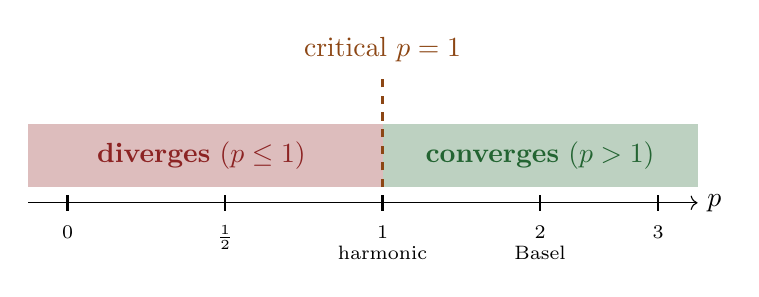
\begin{tikzpicture}[scale=1.0]
    % Horizontal axis: p
    \draw[->] (-0.5,0) -- (8,0) node[right]{$p$};
    \foreach \p/\lab in {0/0, 2/{\tfrac{1}{2}}, 4/1, 6/2, 7.5/3} {
      \draw[thick] (\p,-0.1) -- (\p,0.1);
      \node[below=2pt] at (\p,-0.1) {\scriptsize $\lab$};
    }

    % Divergent region: p <= 1
    \fill[thmcolor!30] (-0.5,0.2) rectangle (4,1.0);
    \node[thmcolor] at (1.7,0.6) {\textbf{diverges} ($p \leq 1$)};

    % Convergent region: p > 1
    \fill[proofcolor!30] (4,0.2) rectangle (8,1.0);
    \node[proofcolor] at (6,0.6) {\textbf{converges} ($p > 1$)};

    % Critical boundary
    \draw[very thick, mAccent, dashed] (4,0.2) -- (4,1.6);
    \node[mAccent, above=2pt] at (4,1.6) {critical $p = 1$};

    % Annotations under p-axis
    \node[below=12pt] at (4,0) {\scriptsize harmonic};
    \node[below=12pt] at (6,0) {\scriptsize Basel};
  \end{tikzpicture}
  \end{center}

  \vspace{0.4em}
  \begin{center}
    \hl{The boundary $p = 1$ \emph{belongs to the divergent side}.}
  \end{center}

  \note{
    Here is the landscape of the "p"-series at a glance. The
    horizontal axis is the exponent "p". On the left, in red, is
    the region where the series diverges, namely "p" at most 1.
    On the right, in green, is the region where the series
    converges, namely "p" strictly greater than 1. The orange
    dashed line at "p" equals 1 is the critical boundary, and
    crucially, the boundary itself belongs to the divergent side.
    The harmonic series, sitting right at "p" equals 1, just
    barely fails to converge. The Basel series, at "p" equals 2,
    is safely inside the convergent region.
  }
\end{frame}
}

{
\usebackgroundtemplate{%
  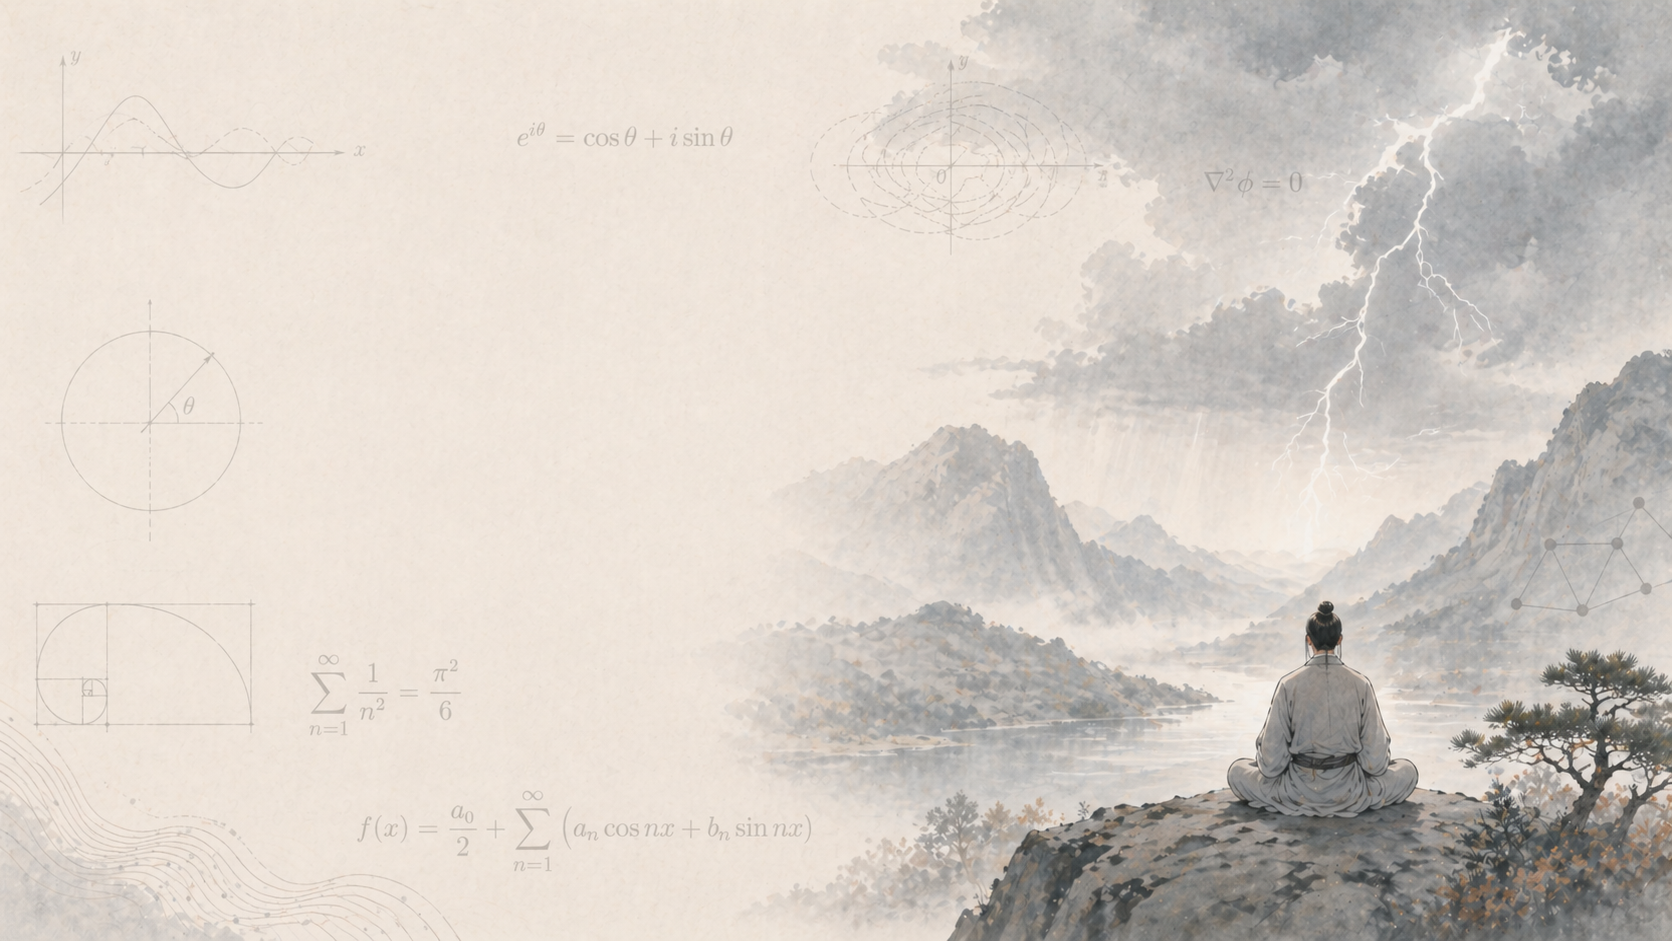
\includegraphics[width=\paperwidth,height=\paperheight,keepaspectratio=false]{chapter_03_bg_05.png}%
}
% =============================================================================
% LOGARITHMIC SERIES
% =============================================================================
\section{Logarithmic Series}

% --- Remark on log ---
\begin{frame}{A Note on $\log n$}
  \begin{remblock}{Remark}
    Throughout, $\log n$ denotes the \emph{natural logarithm} of $n$
    (logarithm to the base $e$; compare Exercise 7, Chap.\ 1).

    \vspace{0.3em}
    The number $e$ will be defined shortly (Definition 3.30).
    We start the series at $n = 2$, since $\log 1 = 0$.
  \end{remblock}

  \note{
    Before stating the next theorem, a small note about notation.
    In this book the symbol "log" always means the natural
    logarithm, that is, logarithm to the base "e". This is
    consistent with most analysis texts. The number "e" itself is
    defined in the next section, but its existence is not needed
    for what follows: we only use that the logarithm is a
    monotonically increasing function. Notice also that the series
    has to start at "n" equal to 2, because at "n" equal to 1 the
    logarithm is zero and we would be dividing by zero.
  }
\end{frame}

% --- Theorem 3.29 ---
\begin{frame}{Theorem 3.29: Logarithmic $p$-Series}
  \begin{thmblock}{Theorem 3.29}
    If $p > 1$, the series
    \[
      \sum_{n=2}^{\infty} \frac{1}{n\, (\log n)^p} \tag{10}
    \]
    converges. If $p \leq 1$, the series diverges.
  \end{thmblock}

  \vspace{0.6em}
  \begin{hlbox}
    Same threshold $p = 1$ as in Theorem 3.28 --- but with an extra log in the denominator.
  \end{hlbox}

  \note{
    Theorem 3.29 is a more refined cousin of the "p"-series test.
    The terms are 1 over "n" times log of "n" to the "p" power,
    which is smaller than 1 over "n" to the "p" but only barely:
    the extra logarithm factor decays very slowly. Remarkably, the
    threshold is exactly the same as in Theorem 3.28. The series
    converges if and only if "p" is strictly greater than 1.
  }
\end{frame}

% --- Proof ---
\begin{frame}{Proof of Theorem 3.29}
  \begin{proofblock}{Apply Cauchy condensation again}
    The logarithm is monotonically increasing, so
    $\{1/(n \log n)\}$ \emph{decreases}. Theorem 3.27 applies. The
    condensed series is
    \begin{equation*}
      \sum_{k=1}^{\infty} 2^k \cdot \frac{1}{2^k \,(\log 2^k)^p}
      \;=\; \sum_{k=1}^{\infty} \frac{1}{(k \log 2)^p}
      \;=\; \frac{1}{(\log 2)^p}\, \sum_{k=1}^{\infty} \frac{1}{k^p} . \tag{11}
    \end{equation*}
  \end{proofblock}

  \vspace{0.4em}
  \hl{A constant times a $p$-series. \alert{Theorem 3.28} delivers the verdict.} \hfill $\square$

  \note{
    The proof is one line of algebra. The logarithm is increasing,
    so its reciprocal is decreasing, and the whole sequence 1 over
    "n" log "n" decreases. So Cauchy condensation applies. Plug in
    "a" sub 2 to the "k" equals 1 over 2 to the "k" times log of 2
    to the "k" to the "p" power. The factor 2 to the "k" outside
    cancels the 2 to the "k" inside, the log of 2 to the "k"
    simplifies to "k" times log 2, and we are left with a constant
    times the sum of 1 over "k" to the "p". By the "p"-series test
    that converges if and only if "p" is greater than 1, and the
    theorem follows.
  }
\end{frame}

% --- Iterated examples build 1 ---
\begin{frame}{The Procedure Continues}
  \hl{\textbf{Plugging more log factors into the denominator:}}

  \vspace{0.5em}
  \begin{exblock}{Example: equation (12)}
    \[
      \sum_{n=3}^{\infty} \frac{1}{n \log n \,\log\log n}
      \quad \alert{\textbf{diverges}}.
    \]
  \end{exblock}

  \note{
    The condensation trick is not a one-shot device; it can be
    applied again and again. Start from the borderline divergent
    series, 1 over "n" times log "n", and slip one more slowly
    growing factor, the log of log "n", into the denominator. That
    gives the series on the slide, equation 12. You might hope
    that this extra factor finally tames the divergence, since it
    makes the terms even smaller. It does not. Running the
    condensation argument one more time reduces equation 12 to a
    harmonic-type series, which we already know diverges. So
    equation 12 diverges as well, even though its terms shrink
    faster than those of any divergent "p"-series.
  }
\end{frame}

% --- Iterated examples build 2 ---
\begin{frame}{The Procedure Continues}
  \hl{\textbf{Plugging more log factors into the denominator:}}

  \vspace{0.5em}
  \begin{exblock}{Example: equation (12)}
    \[
      \sum_{n=3}^{\infty} \frac{1}{n \log n \,\log\log n}
      \quad \alert{\textbf{diverges}}.
    \]
  \end{exblock}

  \vspace{0.4em}
  \begin{exblock}{Example: equation (13)}
    \[
      \sum_{n=3}^{\infty} \frac{1}{n \log n \,(\log\log n)^2}
      \quad \alert{\textbf{converges}}.
    \]
  \end{exblock}

  \note{
    But if we square the iterated logarithm, we tip over into
    convergence. The series in equation 13 converges, again by the
    same condensation argument reducing to a "p"-series with
    exponent 2. So the procedure tells us, by iteration, exactly
    where the borderline is at each level of nested logarithms.
  }
\end{frame}
}

{
\usebackgroundtemplate{%
  
\includegraphics[width=\paperwidth,height=\paperheight,keepaspectratio=false]{chapter_03_bg_06.png}%
}
% =============================================================================
% THE ELUSIVE BOUNDARY
% =============================================================================
\section{The Elusive Boundary}

% --- Build 1/3 ---
\begin{frame}{Is There a Sharp Boundary?}
  \begin{hlbox}
  \begin{itemize}
    \item Equations (12) and (13) differ only by an extra factor of $\log\log n$.
    \item One diverges, the other converges.
  \end{itemize}
  \end{hlbox}

  \note{
    Look closely at the two examples we just saw. Their terms
    differ only by an extra factor of log log "n". Yet one
    diverges and the other converges. The gap between divergence
    and convergence is incredibly thin.
  }
\end{frame}

% --- Build 2/3 ---
\begin{frame}{Is There a Sharp Boundary?}
  \begin{hlbox}
  \begin{itemize}
    \item Equations (12) and (13) differ only by an extra factor of $\log\log n$.
    \item One diverges, the other converges.
    \item Iterating the procedure: even thinner gaps appear.
  \end{itemize}
  \end{hlbox}

  \note{
    Worse, we can iterate the trick. Sticking in more nested
    logarithms produces matched pairs of divergent and convergent
    series whose terms differ by less and less. The natural
    question is: is there some ultimate borderline series, a
    convergent series whose terms are larger than every divergent
    series in this family?
  }
\end{frame}

% --- Build 3/3 ---
\begin{frame}{Is There a Sharp Boundary?}
  \begin{hlbox}
  \begin{itemize}
    \item Equations (12) and (13) differ only by an extra factor of $\log\log n$.
    \item One diverges, the other converges.
    \item Iterating the procedure: even thinner gaps appear.
    \item \alert{No} such boundary exists --- See Exercises 11(b), 12(b).
  \end{itemize}
  \end{hlbox}

  \vspace{0.5em}
  \begin{remblock}{Knopp reference}
    See Knopp, \emph{Theory and Application of Infinite Series},
    Ch.\ IX, Sec.\ 41, for a fuller treatment.
  \end{remblock}

  \note{
    The answer is no. No matter how we try to make the notion of a
    boundary precise, no such boundary exists. There is no slowest
    convergent series, and no fastest divergent series, even among
    monotone series. Exercises 11 part "b" and 12 part "b" in this
    chapter sketch one way to make that statement precise. For a
    deeper discussion, Rudin points readers to Knopp's classic book
    on infinite series, particularly chapter 9, section 41.
  }
\end{frame}
}

{
\usebackgroundtemplate{%
  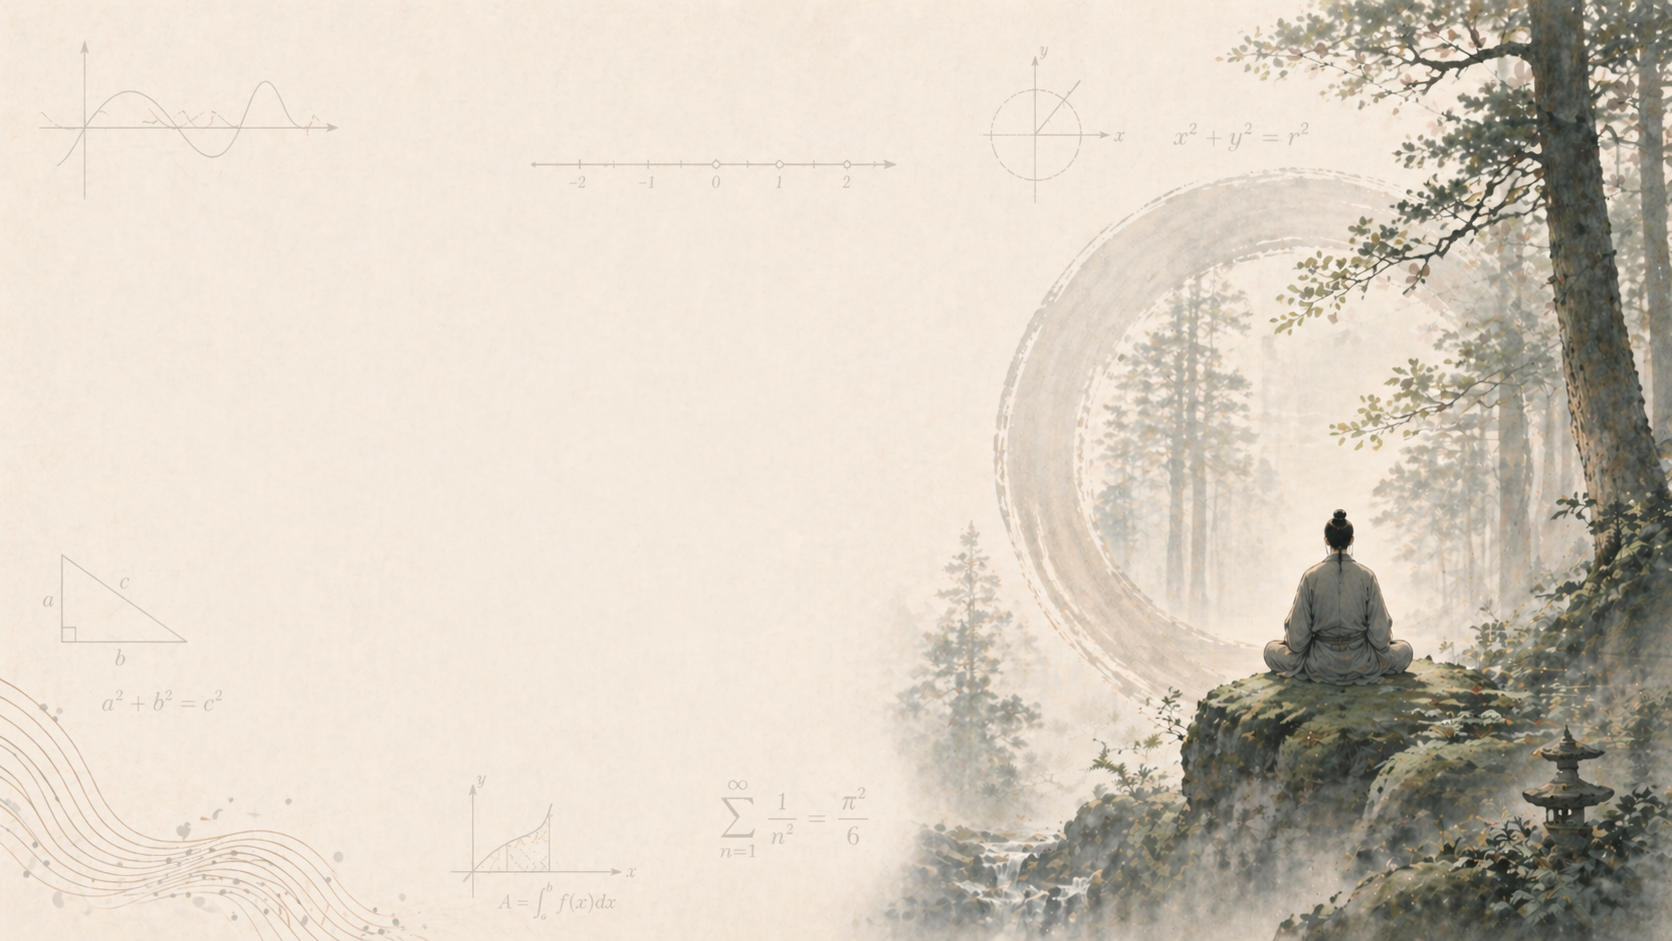
\includegraphics[width=\paperwidth,height=\paperheight,keepaspectratio=false]{chapter_03_bg_07.png}%
}
% =============================================================================
% SUMMARY
% =============================================================================
\section{Summary}

% --- Build 1/4 ---
\begin{frame}{Summary}
  \begin{hlbox}
  \textbf{Key takeaways:}
  \begin{itemize}
    \item \alert{Theorem 3.26 (geometric)}: $\sum x^n \to 1/(1-x)$ iff $0 \leq x < 1$.
  \end{itemize}
  \end{hlbox}

  \note{
    Let us review what we have collected. First, the geometric
    series, our most basic reference. It converges for "x" in the
    interval from 0 to 1, not including 1, and diverges otherwise.
    When it converges, we know its sum explicitly: 1 over 1 minus
    "x". This is the only one of our reference series for which
    we have a closed-form sum.
  }
\end{frame}

% --- Build 2/4 ---
\begin{frame}{Summary}
  \begin{hlbox}
  \textbf{Key takeaways:}
  \begin{itemize}
    \item \alert{Theorem 3.26 (geometric)}: $\sum x^n \to 1/(1-x)$ iff $0 \leq x < 1$.
    \item \alert{Theorem 3.27 (Cauchy condensation)}: for $a_n \downarrow 0$,
      $\;\sum a_n$ and $\sum 2^k a_{2^k}$ converge (or diverge) together.
  \end{itemize}
  \end{hlbox}

  \note{
    Second, the Cauchy condensation test. For nonnegative
    decreasing terms, the original series and the condensed
    series, sampled at powers of 2, converge together. This is
    the engine that drives the rest of the section: it converts
    questions about slow-decaying series into questions about
    geometric or "p"-type series.
  }
\end{frame}

% --- Build 3/4 ---
\begin{frame}{Summary}
  \begin{hlbox}
  \textbf{Key takeaways:}
  \begin{itemize}
    \item \alert{Theorem 3.26 (geometric)}: $\sum x^n \to 1/(1-x)$ iff $0 \leq x < 1$.
    \item \alert{Theorem 3.27 (Cauchy condensation)}: for $a_n \downarrow 0$,
      $\;\sum a_n$ and $\sum 2^k a_{2^k}$ converge (or diverge) together.
    \item \alert{Theorem 3.28 ($p$-series)}: $\sum 1/n^p$ converges iff $p > 1$.
  \end{itemize}
  \end{hlbox}

  \note{
    Third, the "p"-series test. The series 1 over "n" to the "p"
    converges precisely when "p" is strictly greater than 1. The
    harmonic series, at "p" equals 1, just barely fails to
    converge, and this fact will haunt us many times in the rest
    of the book.
  }
\end{frame}

% --- Build 4/4 ---
\begin{frame}{Summary}
  \begin{hlbox}
  \textbf{Key takeaways:}
  \begin{itemize}
    \item \alert{Theorem 3.26 (geometric)}: $\sum x^n \to 1/(1-x)$ iff $0 \leq x < 1$.
    \item \alert{Theorem 3.27 (Cauchy condensation)}: for $a_n \downarrow 0$,
      $\;\sum a_n$ and $\sum 2^k a_{2^k}$ converge (or diverge) together.
    \item \alert{Theorem 3.28 ($p$-series)}: $\sum 1/n^p$ converges iff $p > 1$.
    \item \alert{Theorem 3.29 (logarithmic)}: $\sum 1/(n (\log n)^p)$ converges iff $p > 1$.
  \end{itemize}
  \end{hlbox}

  \vspace{0.6em}
  \begin{hlbox}
    \textbf{Coming up next:} Definition of the number $e$ and a careful estimate of its irrationality.
  \end{hlbox}

  \note{
    Fourth, the logarithmic series. Inserting a log "n" to the
    "p" factor in the denominator shifts the threshold downward
    only slightly: the cutoff is still "p" equals 1. We also saw
    that the procedure iterates indefinitely, with no ultimate
    boundary between convergent and divergent series. Coming up
    next: the number "e" gets its definition, and we estimate
    just how badly it fails to be a rational number. That sets
    the stage for the root and ratio tests later in the chapter.
  }
\end{frame}
}

\end{document}
